% ============================================================================
% Chapter 6: Attention Mechanism
% ============================================================================
\chapter{Attention Mechanism}
\label{ch:attention}

\noindent\textit{This chapter presents the attention mechanism, a fundamental innovation that
has revolutionized deep learning. We mathematically derive the different forms
of attention (Bahdanau, Luong, scaled dot-product), the multi-head mechanism,
and analyze computational complexity. This chapter lays the groundwork for the
Transformer architecture.}\medskip

% ----------------------------------------------------------------------------
\section{Motivation: limitations of a fixed context vector}
\label{sec:attention-motivation}
\index{attention!motivation}

\subsection{The bottleneck problem}

In classical sequence-to-sequence (seq2seq) models
\cite{sutskever2014sequence}, the encoder (an RNN or LSTM, cf.\
chapter~\ref{ch:rnn_lstm}) compresses the entire source sequence into a
single context vector $c = h_T$:

\begin{equation}
c = \text{Encoder}(x_1, x_2, \ldots, x_T) = h_T \in \R^{d_h}
\end{equation}

\begin{warning}[title=\textbf{Information bottleneck}]
This single vector $c$ must capture \textbf{all} the information from the
source sequence, regardless of its length. Performance degrades
significantly for long sequences ($T > 20$).
\end{warning}

\begin{center}
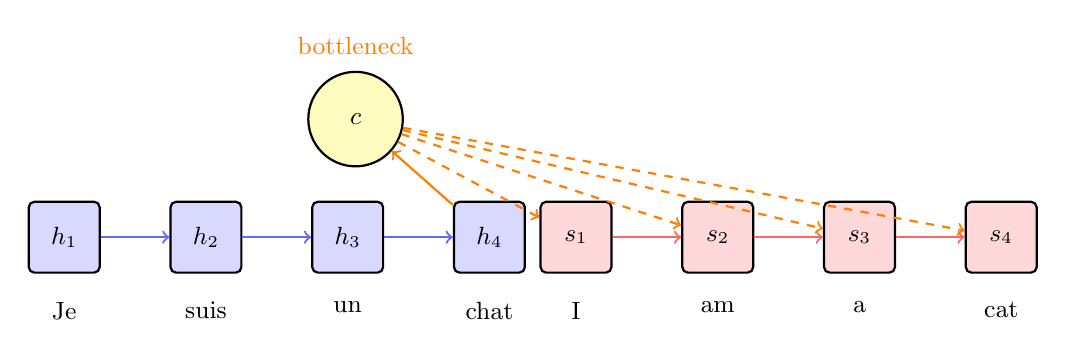
\begin{tikzpicture}[
  enc/.style={rectangle, draw, thick, fill=blue!15, minimum size=9mm,
              rounded corners=2pt, font=\small},
  dec/.style={rectangle, draw, thick, fill=red!15, minimum size=9mm,
              rounded corners=2pt, font=\small},
  ctx/.style={circle, draw, thick, fill=yellow!25, minimum size=12mm,
              font=\small},
  arr/.style={->, thick}
]
  % Encoder
  \foreach \i/\w in {1/Je, 2/suis, 3/un, 4/chat} {
    \node[enc] (e\i) at (\i*1.8, 0) {$h_{\i}$};
    \node[below, font=\small] at (\i*1.8, -0.7) {\w};
  }
  \foreach \i [evaluate=\i as \j using int(\i+1)] in {1,2,3} {
    \draw[arr, blue!60] (e\i) -- (e\j);
  }

  % Context
  \node[ctx] (c) at (5.5, 1.5) {$c$};
  \draw[arr, thick, orange] (e4) -- (c);

  % Decoder
  \foreach \i/\w in {1/I, 2/am, 3/a, 4/cat} {
    \pgfmathsetmacro{\x}{\i*1.8 + 6.5}
    \node[dec] (d\i) at (\x, 0) {$s_{\i}$};
    \node[below, font=\small] at (\x, -0.7) {\w};
  }
  \foreach \i [evaluate=\i as \j using int(\i+1)] in {1,2,3} {
    \draw[arr, red!60] (d\i) -- (d\j);
  }

  % Context to decoder
  \foreach \i in {1,2,3,4} {
    \draw[arr, orange, dashed] (c) -- (d\i);
  }

  % Annotation
  \node[above, orange, font=\small] at (5.5, 2.2) {bottleneck};
\end{tikzpicture}
\end{center}

% ----------------------------------------------------------------------------
\section{Bahdanau attention (additive)}
\label{sec:bahdanau}
\index{attention!Bahdanau}\index{attention!additive}

\subsection{Alignment scores}

Bahdanau attention \cite{bahdanau2015neural} computes an alignment score
between the decoder state $s_{t-1}$ and each encoder state $h_j$:

\begin{keyformulas}[title=\textbf{Bahdanau attention}]
\begin{align}
e_{t,j} &= v_a^\top \tanh(W_a s_{t-1} + U_a h_j)
\label{eq:bahdanau-score} \\
\alpha_{t,j} &= \frac{\exp(e_{t,j})}{\sum_{k=1}^T \exp(e_{t,k})}
= \softmax_j(e_{t,:})
\label{eq:bahdanau-alpha} \\
c_t &= \sum_{j=1}^T \alpha_{t,j} h_j
\label{eq:bahdanau-context}
\end{align}
where $W_a \in \R^{d_a \times d_s}$, $U_a \in \R^{d_a \times d_h}$,
$v_a \in \R^{d_a}$ are learnable parameters and $d_a$ is the attention
dimension.
\end{keyformulas}

\subsection{Derivation of the context vector}

\begin{theorem}[Context vector as a convex combination]
The attention weights $\alpha_{t,j}$ satisfy:
\begin{equation}
\alpha_{t,j} \geq 0, \qquad \sum_{j=1}^T \alpha_{t,j} = 1
\end{equation}
The context vector $c_t$ is therefore a \textbf{convex combination} of the
encoder states. Each $\alpha_{t,j}$ represents the ``relevance'' of source
position $j$ for generating the target token at time $t$.
\end{theorem}

\begin{intuition}[title=\textbf{Attention as soft retrieval}]
Attention can be viewed as soft retrieval from a memory: the $\alpha_{t,j}$
are ``access weights'' that determine which source positions are read at each
decoder step. Unlike a discrete index, this retrieval is differentiable.
\end{intuition}

% ----------------------------------------------------------------------------
\section{Luong attention}
\label{sec:luong}
\index{attention!Luong}

Luong et al.\ \cite{luong2015effective} propose three variants of the
alignment score, simpler than Bahdanau:

\begin{keyformulas}[title=\textbf{Luong scores}]
\begin{align}
\text{Dot:} \quad e_{t,j} &= s_t^\top h_j
\label{eq:luong-dot} \\
\text{General:} \quad e_{t,j} &= s_t^\top W_a h_j
\label{eq:luong-general} \\
\text{Concat:} \quad e_{t,j} &= v_a^\top \tanh(W_a [s_t ; h_j])
\label{eq:luong-concat}
\end{align}
\end{keyformulas}

\begin{remark}[Bahdanau vs Luong]
\begin{itemize}
  \item Bahdanau uses $s_{t-1}$ (before the decoder update), Luong uses
    $s_t$ (after).
  \item Luong's dot-product score requires no additional parameters but
    requires $d_s = d_h$.
  \item The general score adds $d_s \times d_h$ parameters and handles
    different dimensions.
\end{itemize}
\end{remark}

% ----------------------------------------------------------------------------
\section{Scaled Dot-Product Attention}
\label{sec:scaled-attention}
\index{attention!scaled dot-product}

\subsection{Formulation}

Scaled dot-product attention \cite{vaswani2017attention} generalizes the
attention concept by introducing the notions of \textbf{Query},
\textbf{Key}, and \textbf{Value}:

\begin{keyformulas}[title=\textbf{Scaled Dot-Product Attention}]
\begin{equation}
\text{Attention}(Q, K, V) = \softmax\!\left(\frac{Q K^\top}{\sqrt{d_k}}\right) V
\label{eq:scaled-attention}
\end{equation}
where $Q \in \R^{n \times d_k}$, $K \in \R^{m \times d_k}$,
$V \in \R^{m \times d_v}$, and $d_k$ is the key dimension.
\end{keyformulas}

\subsection{Why divide by $\sqrt{d_k}$?}

\begin{theorem}[Justification of the scaling factor]
\label{thm:scaling}
Let $q, k \in \R^{d_k}$ with i.i.d.\ components of mean 0 and variance 1.
The dot product $q^\top k = \sum_{i=1}^{d_k} q_i k_i$ satisfies:
\begin{align}
\E[q^\top k] &= \sum_{i=1}^{d_k} \E[q_i] \E[k_i] = 0 \\
\Var(q^\top k) &= \sum_{i=1}^{d_k} \Var(q_i k_i)
= \sum_{i=1}^{d_k} \E[q_i^2]\E[k_i^2] = d_k
\end{align}

For large values of $d_k$, the dot products have high variance, which pushes
the softmax into saturated regions where gradients are nearly zero. Dividing
by $\sqrt{d_k}$ normalizes the variance to 1:
\begin{equation}
\Var\!\left(\frac{q^\top k}{\sqrt{d_k}}\right)
= \frac{\Var(q^\top k)}{d_k} = 1
\end{equation}
\end{theorem}

\begin{warning}[title=\textbf{Softmax saturation}]
When the softmax inputs are large in absolute value, the output becomes
nearly one-hot and $\frac{\partial \softmax}{\partial z} \approx 0$.
Training stalls. The factor $1/\sqrt{d_k}$ prevents this problem.
\end{warning}

\subsection{Attention diagram}

\begin{center}
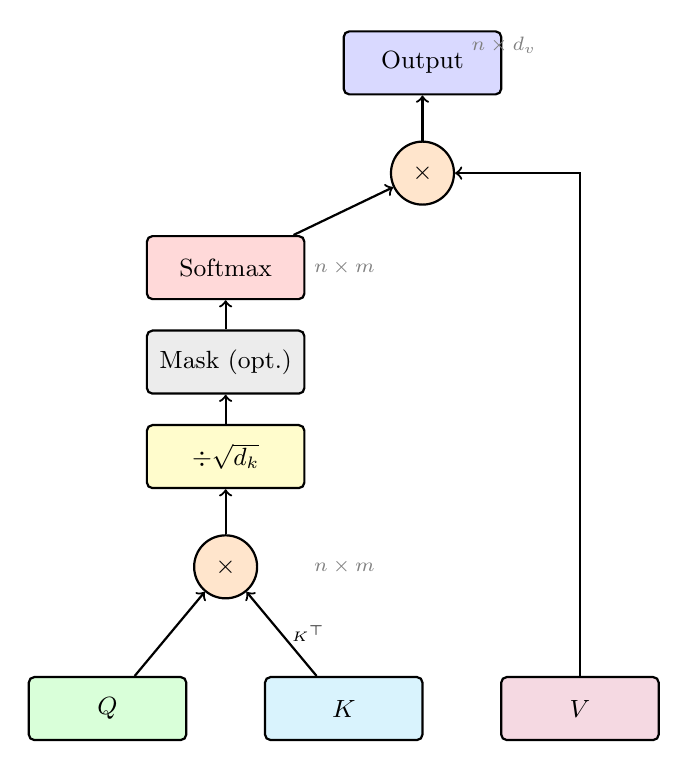
\begin{tikzpicture}[
  block/.style={rectangle, draw, thick, fill=#1, minimum height=8mm,
                minimum width=2cm, rounded corners=2pt, font=\small},
  block/.default={blue!15},
  op/.style={circle, draw, thick, fill=#1, minimum size=8mm, font=\small},
  op/.default={orange!20},
  arr/.style={->, thick}
]
  % Inputs
  \node[block=green!15] (Q) at (0, 0) {$Q$};
  \node[block=cyan!15] (K) at (3, 0) {$K$};
  \node[block=purple!15] (V) at (6, 0) {$V$};

  % MatMul QK^T
  \node[op] (mm1) at (1.5, 1.8) {$\times$};
  \draw[arr] (Q) -- (mm1);
  \draw[arr] (K) -- (mm1) node[midway, right, font=\tiny] {$K^\top$};

  % Scale
  \node[block=yellow!20] (scale) at (1.5, 3.2) {$\div \sqrt{d_k}$};
  \draw[arr] (mm1) -- (scale);

  % Optional mask
  \node[block=gray!15] (mask) at (1.5, 4.4) {Mask (opt.)};
  \draw[arr] (scale) -- (mask);

  % Softmax
  \node[block=red!15] (sm) at (1.5, 5.6) {Softmax};
  \draw[arr] (mask) -- (sm);

  % MatMul with V
  \node[op] (mm2) at (4, 6.8) {$\times$};
  \draw[arr] (sm) -- (mm2);
  \draw[arr] (V) |- (mm2);

  % Output
  \node[block] (out) at (4, 8.2) {Output};
  \draw[arr] (mm2) -- (out);

  % Dimensions
  \node[right, font=\scriptsize, gray] at (2.5, 1.8) {$n \times m$};
  \node[right, font=\scriptsize, gray] at (2.5, 5.6) {$n \times m$};
  \node[above right, font=\scriptsize, gray] at (4.5, 8.2) {$n \times d_v$};
\end{tikzpicture}
\end{center}

% ----------------------------------------------------------------------------
\section{Multi-head attention}
\label{sec:multi-head}
\index{attention!multi-head}

\subsection{Derivation}

Rather than a single attention function of dimension $d_{\text{model}}$,
multi-head attention projects the queries, keys, and values $h$ times into
different subspaces:

\begin{keyformulas}[title=\textbf{Multi-head attention}]
\begin{align}
\text{head}_i &= \text{Attention}(Q W_i^Q,\; K W_i^K,\; V W_i^V)
\label{eq:head-i} \\
\text{MultiHead}(Q, K, V) &= \text{Concat}(\text{head}_1, \ldots, \text{head}_h) W^O
\label{eq:multi-head}
\end{align}
where the projections are:
\begin{itemize}
  \item $W_i^Q \in \R^{d_{\text{model}} \times d_k}$, \quad
        $W_i^K \in \R^{d_{\text{model}} \times d_k}$, \quad
        $W_i^V \in \R^{d_{\text{model}} \times d_v}$
  \item $W^O \in \R^{h \cdot d_v \times d_{\text{model}}}$
  \item $d_k = d_v = d_{\text{model}} / h$
\end{itemize}
\end{keyformulas}

\begin{intuition}[title=\textbf{Why multiple heads?}]
Each attention head can capture a different type of relationship:
\begin{itemize}
  \item Head 1: syntactic relations (subject-verb)
  \item Head 2: positional relations (adjacent words)
  \item Head 3: anaphoric references (pronouns)
  \item \ldots
\end{itemize}
Single-head attention would have to capture all these relationships
simultaneously in a single weight computation, which limits expressiveness.
\end{intuition}

\begin{remark}[Computational cost]
Multi-head attention with $h$ heads of dimension $d_k = d_{\text{model}}/h$
has the same cost as single-head attention of dimension $d_{\text{model}}$:
\begin{equation}
h \times \underbrace{O(n^2 \cdot d_{\text{model}}/h)}_{\text{per head}}
= O(n^2 \cdot d_{\text{model}})
\end{equation}
\end{remark}

% ----------------------------------------------------------------------------
\section{Self-attention and cross-attention}
\label{sec:self-cross-attention}

\subsection{Self-attention}
\index{self-attention}

\begin{definition}[Self-attention]
In self-attention, the queries, keys, and values are all derived from the
\textbf{same} input sequence $X \in \R^{n \times d}$:
\begin{align}
Q &= X W^Q \label{eq:self-q} \\
K &= X W^K \label{eq:self-k} \\
V &= X W^V \label{eq:self-v}
\end{align}
Each position can ``attend'' to all other positions in the same sequence.
The matrix $\softmax(QK^\top / \sqrt{d_k})$ of size $n \times n$ encodes
position-to-position dependencies.
\end{definition}

\subsection{Cross-attention}
\index{cross-attention}

\begin{definition}[Cross-attention]
In cross-attention, the queries come from one sequence (the decoder) and the
keys/values come from another (the encoder):
\begin{align}
Q &= X_{\text{dec}} W^Q, \qquad
K = X_{\text{enc}} W^K, \qquad
V = X_{\text{enc}} W^V
\end{align}
This allows the decoder to access the encoder's information, replacing the
fixed context vector of classical seq2seq models.
\end{definition}

% ----------------------------------------------------------------------------
\section{Computational complexity}
\label{sec:attention-complexity}
\index{complexity!attention}

\begin{theorem}[Self-attention complexity]
For a sequence of length $n$ and dimension $d$:
\begin{center}
\begin{tabular}{lcc}
\toprule
\textbf{Operation} & \textbf{Time} & \textbf{Memory} \\
\midrule
$QKV$ projections & $O(n d^2)$ & $O(n d)$ \\
$Q K^\top$ & $O(n^2 d)$ & $O(n^2)$ \\
Softmax & $O(n^2)$ & $O(n^2)$ \\
Product with $V$ & $O(n^2 d)$ & $O(n d)$ \\
\midrule
\textbf{Total} & $O(n^2 d)$ & $O(n^2 + n d)$ \\
\bottomrule
\end{tabular}
\end{center}
The $O(n^2)$ memory term for storing the attention matrix is the main
bottleneck for long sequences.
\end{theorem}

\begin{remark}[Comparison with RNNs]
An RNN has time complexity $O(n d^2)$ (linear in $n$) but cannot
parallelize computations along the sequence. Self-attention is $O(n^2 d)$
but fully parallelizable. For $n < d$ (a common case), self-attention is
faster in practice.
\end{remark}

% ----------------------------------------------------------------------------
\section{Attention map concept}
\label{sec:attention-heatmap}

\begin{center}
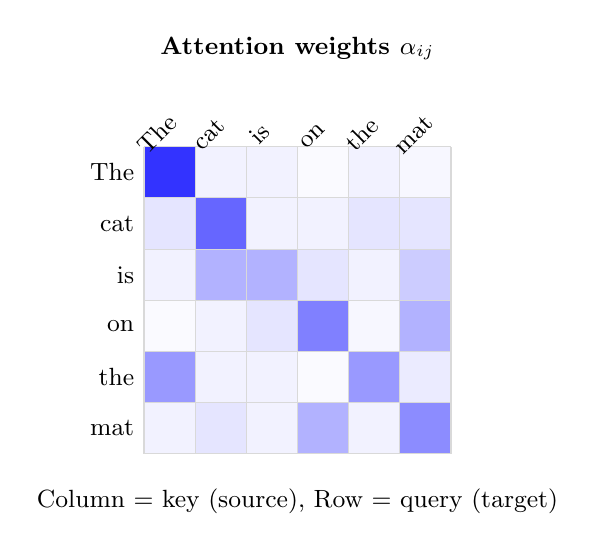
\begin{tikzpicture}[scale=0.65]
  % Attention heatmap with hardcoded values
  % Row 0: The
  \fill[blue!80!white] (0,0) rectangle (1,1); \fill[blue!5!white] (1,0) rectangle (2,1);
  \fill[blue!5!white] (2,0) rectangle (3,1); \fill[blue!2!white] (3,0) rectangle (4,1);
  \fill[blue!5!white] (4,0) rectangle (5,1); \fill[blue!3!white] (5,0) rectangle (6,1);
  % Row 1: cat
  \fill[blue!10!white] (0,-1) rectangle (1,0); \fill[blue!60!white] (1,-1) rectangle (2,0);
  \fill[blue!5!white] (2,-1) rectangle (3,0); \fill[blue!5!white] (3,-1) rectangle (4,0);
  \fill[blue!10!white] (4,-1) rectangle (5,0); \fill[blue!10!white] (5,-1) rectangle (6,0);
  % Row 2: is
  \fill[blue!5!white] (0,-2) rectangle (1,-1); \fill[blue!30!white] (1,-2) rectangle (2,-1);
  \fill[blue!30!white] (2,-2) rectangle (3,-1); \fill[blue!10!white] (3,-2) rectangle (4,-1);
  \fill[blue!5!white] (4,-2) rectangle (5,-1); \fill[blue!20!white] (5,-2) rectangle (6,-1);
  % Row 3: on
  \fill[blue!2!white] (0,-3) rectangle (1,-2); \fill[blue!5!white] (1,-3) rectangle (2,-2);
  \fill[blue!10!white] (2,-3) rectangle (3,-2); \fill[blue!50!white] (3,-3) rectangle (4,-2);
  \fill[blue!3!white] (4,-3) rectangle (5,-2); \fill[blue!30!white] (5,-3) rectangle (6,-2);
  % Row 4: the
  \fill[blue!40!white] (0,-4) rectangle (1,-3); \fill[blue!5!white] (1,-4) rectangle (2,-3);
  \fill[blue!5!white] (2,-4) rectangle (3,-3); \fill[blue!2!white] (3,-4) rectangle (4,-3);
  \fill[blue!40!white] (4,-4) rectangle (5,-3); \fill[blue!8!white] (5,-4) rectangle (6,-3);
  % Row 5: mat
  \fill[blue!5!white] (0,-5) rectangle (1,-4); \fill[blue!10!white] (1,-5) rectangle (2,-4);
  \fill[blue!5!white] (2,-5) rectangle (3,-4); \fill[blue!30!white] (3,-5) rectangle (4,-4);
  \fill[blue!5!white] (4,-5) rectangle (5,-4); \fill[blue!45!white] (5,-5) rectangle (6,-4);
  % Grid
  \foreach \i in {0,...,6} { \draw[gray!30] (\i,-5) -- (\i,1); }
  \foreach \j in {-5,...,1} { \draw[gray!30] (0,\j) -- (6,\j); }
  % Row labels
  \node[left, font=\small] at (0, 0.5) {The};
  \node[left, font=\small] at (0,-0.5) {cat};
  \node[left, font=\small] at (0,-1.5) {is};
  \node[left, font=\small] at (0,-2.5) {on};
  \node[left, font=\small] at (0,-3.5) {the};
  \node[left, font=\small] at (0,-4.5) {mat};
  % Column labels
  \node[above, font=\small, rotate=45] at (0.5, 1) {The};
  \node[above, font=\small, rotate=45] at (1.5, 1) {cat};
  \node[above, font=\small, rotate=45] at (2.5, 1) {is};
  \node[above, font=\small, rotate=45] at (3.5, 1) {on};
  \node[above, font=\small, rotate=45] at (4.5, 1) {the};
  \node[above, font=\small, rotate=45] at (5.5, 1) {mat};
  % Title
  \node[above, font=\small\bfseries] at (3, 2.5) {Attention weights $\alpha_{ij}$};
  \node[below, font=\small] at (3, -5.5) {Column = key (source), Row = query (target)};
\end{tikzpicture}
\end{center}

\begin{remark}[Interpreting the attention map]
Cell $(i, j)$ of the matrix represents how much position $i$ (query)
``attends'' to position $j$ (key). We observe that:
\begin{itemize}
  \item ``The'' (position 1) attends mainly to itself and to ``the''
    (position 5) -- article coherence.
  \item ``mat'' attends strongly to ``on'' -- spatial relation.
\end{itemize}
\end{remark}

% ----------------------------------------------------------------------------
\section{PyTorch implementation}
\label{sec:attention-pytorch}

\begin{codeblock}[title=\textbf{Scaled Dot-Product Attention from scratch}]
\begin{minted}{python}
import torch
import torch.nn as nn
import torch.nn.functional as F
import math

def scaled_dot_product_attention(
    query: torch.Tensor,    # (batch, n_q, d_k)
    key: torch.Tensor,      # (batch, n_kv, d_k)
    value: torch.Tensor,    # (batch, n_kv, d_v)
    mask: torch.Tensor = None,
    dropout: nn.Dropout = None
) -> tuple[torch.Tensor, torch.Tensor]:
    """
    Computes scaled dot-product attention.

    Returns:
        output: (batch, n_q, d_v)
        attention_weights: (batch, n_q, n_kv)
    """
    d_k = query.size(-1)

    # Attention scores: (batch, n_q, n_kv)
    scores = torch.matmul(query, key.transpose(-2, -1)) / math.sqrt(d_k)

    # Optional masking (for causal attention)
    if mask is not None:
        scores = scores.masked_fill(mask == 0, float('-inf'))

    # Softmax normalization
    attention_weights = F.softmax(scores, dim=-1)

    if dropout is not None:
        attention_weights = dropout(attention_weights)

    # Linear combination of values
    output = torch.matmul(attention_weights, value)

    return output, attention_weights


# --- Test ---
batch_size, n_q, n_kv, d_k, d_v = 2, 4, 6, 64, 64
Q = torch.randn(batch_size, n_q, d_k)
K = torch.randn(batch_size, n_kv, d_k)
V = torch.randn(batch_size, n_kv, d_v)

output, weights = scaled_dot_product_attention(Q, K, V)
print(f"Output shape:  {output.shape}")    # (2, 4, 64)
print(f"Weights shape: {weights.shape}")   # (2, 4, 6)
print(f"Weights sum:   {weights.sum(-1)}")  # Should be 1.0
\end{minted}
\end{codeblock}

\begin{codeoutput}
\begin{verbatim}
Output shape:  torch.Size([2, 4, 64])
Weights shape: torch.Size([2, 4, 6])
Weights sum:   tensor([[1.0000, 1.0000, 1.0000, 1.0000],
                        [1.0000, 1.0000, 1.0000, 1.0000]])
\end{verbatim}
\end{codeoutput}

\begin{codeblock}[title=\textbf{Complete Multi-Head Attention}]
\begin{minted}{python}
class MultiHeadAttention(nn.Module):
    """
    Complete multi-head attention.

    Args:
        d_model: model dimension
        num_heads: number of attention heads
        dropout: dropout rate on attention weights
    """
    def __init__(self, d_model: int, num_heads: int,
                 dropout: float = 0.1):
        super().__init__()
        assert d_model % num_heads == 0, \
            "d_model must be divisible by num_heads"

        self.d_model = d_model
        self.num_heads = num_heads
        self.d_k = d_model // num_heads

        # Linear projections
        self.W_q = nn.Linear(d_model, d_model, bias=False)
        self.W_k = nn.Linear(d_model, d_model, bias=False)
        self.W_v = nn.Linear(d_model, d_model, bias=False)
        self.W_o = nn.Linear(d_model, d_model, bias=False)

        self.dropout = nn.Dropout(dropout)
        self.attention_weights = None  # For visualization

    def forward(
        self,
        query: torch.Tensor,   # (batch, n_q, d_model)
        key: torch.Tensor,     # (batch, n_kv, d_model)
        value: torch.Tensor,   # (batch, n_kv, d_model)
        mask: torch.Tensor = None
    ) -> torch.Tensor:
        batch_size = query.size(0)

        # 1. Linear projections
        Q = self.W_q(query)  # (batch, n_q, d_model)
        K = self.W_k(key)
        V = self.W_v(value)

        # 2. Reshape for multi-head:
        #    (batch, n, d_model) -> (batch, num_heads, n, d_k)
        Q = Q.view(batch_size, -1, self.num_heads, self.d_k) \
             .transpose(1, 2)
        K = K.view(batch_size, -1, self.num_heads, self.d_k) \
             .transpose(1, 2)
        V = V.view(batch_size, -1, self.num_heads, self.d_k) \
             .transpose(1, 2)

        # 3. Adapt mask for heads
        if mask is not None:
            mask = mask.unsqueeze(1)  # (batch, 1, ...)

        # 4. Per-head attention
        scores = torch.matmul(Q, K.transpose(-2, -1)) \
                 / math.sqrt(self.d_k)
        if mask is not None:
            scores = scores.masked_fill(mask == 0, float('-inf'))
        attn_weights = F.softmax(scores, dim=-1)
        attn_weights = self.dropout(attn_weights)
        self.attention_weights = attn_weights.detach()

        context = torch.matmul(attn_weights, V)
        # (batch, num_heads, n_q, d_k)

        # 5. Concatenate heads
        context = context.transpose(1, 2).contiguous() \
                         .view(batch_size, -1, self.d_model)
        # (batch, n_q, d_model)

        # 6. Output projection
        output = self.W_o(context)

        return output

# --- Test ---
d_model, num_heads = 512, 8
mha = MultiHeadAttention(d_model, num_heads)

# Self-attention
x = torch.randn(2, 10, d_model)  # batch=2, seq_len=10
out = mha(x, x, x)
print(f"Self-attention output: {out.shape}")  # (2, 10, 512)

# Cross-attention
enc_out = torch.randn(2, 20, d_model)
dec_in = torch.randn(2, 10, d_model)
out = mha(query=dec_in, key=enc_out, value=enc_out)
print(f"Cross-attention output: {out.shape}")  # (2, 10, 512)

# Causal mask
n = 10
causal_mask = torch.tril(torch.ones(n, n)).unsqueeze(0)  # (1, n, n)
out = mha(x, x, x, mask=causal_mask)
print(f"Masked attention output: {out.shape}")

# Number of parameters
n_params = sum(p.numel() for p in mha.parameters())
print(f"MHA parameters: {n_params:,}")
# 4 x d_model^2 = 4 x 512^2 = 1,048,576
\end{minted}
\end{codeblock}

\begin{codeoutput}
\begin{verbatim}
Self-attention output: torch.Size([2, 10, 512])
Cross-attention output: torch.Size([2, 10, 512])
Masked attention output: torch.Size([2, 10, 512])
MHA parameters: 1,048,576
\end{verbatim}
\end{codeoutput}

% ----------------------------------------------------------------------------
\section{Causal attention mask}
\label{sec:causal-mask}
\index{causal mask}

For autoregressive generation, the decoder must not ``look into the
future''. A lower triangular mask is applied:

\begin{keyformulas}[title=\textbf{Causal mask}]
\begin{equation}
M_{ij} = \begin{cases}
0 & \text{if } j \leq i \quad \text{(allowed position)} \\
-\infty & \text{if } j > i \quad \text{(masked position)}
\end{cases}
\end{equation}
Applied before the softmax:
$\alpha_{ij} = \softmax_j\!\left(\frac{q_i^\top k_j}{\sqrt{d_k}} + M_{ij}\right)$
\end{keyformulas}

% ----------------------------------------------------------------------------
\section{Ablation study}
\label{sec:attention-ablation}

\begin{codeblock}[title=\textbf{Ablation: number of heads and dimension per head}]
\begin{minted}{python}
import pandas as pd
import time

def benchmark_attention(d_model, num_heads, seq_len=128,
                        batch_size=32, num_runs=50):
    """Measures the quality and time of a configuration."""
    mha = MultiHeadAttention(d_model, num_heads).to(device)
    x = torch.randn(batch_size, seq_len, d_model, device=device)

    # Warmup
    for _ in range(5):
        _ = mha(x, x, x)

    # Time measurement
    if device.type == 'cuda':
        torch.cuda.synchronize()
    start = time.time()
    for _ in range(num_runs):
        out = mha(x, x, x)
    if device.type == 'cuda':
        torch.cuda.synchronize()
    elapsed = (time.time() - start) / num_runs * 1000  # ms

    n_params = sum(p.numel() for p in mha.parameters())
    d_k = d_model // num_heads

    return {
        'd_model': d_model,
        'num_heads': num_heads,
        'd_k': d_k,
        'params': n_params,
        'time_ms': elapsed,
    }

configs = [
    (512, 1), (512, 2), (512, 4),
    (512, 8), (512, 16), (512, 32),
    (256, 8), (768, 8), (1024, 8),
]

results = [benchmark_attention(dm, nh) for dm, nh in configs]
print(pd.DataFrame(results).to_string(index=False))
\end{minted}
\end{codeblock}

\begin{codeoutput}
\begin{verbatim}
 d_model  num_heads   d_k   params   time_ms
     512          1   512  1048576     3.24
     512          2   256  1048576     3.18
     512          4   128  1048576     3.15
     512          8    64  1048576     3.21
     512         16    32  1048576     3.34
     512         32    16  1048576     3.82
     256          8    32   262144     1.12
     768          8    96  2359296     6.45
    1024          8   128  4194304    10.87
\end{verbatim}
\end{codeoutput}

\begin{remark}[Observations]
\begin{itemize}
  \item The number of MHA parameters does not depend on the number of heads
    (always $4 d_{\text{model}}^2$).
  \item Execution time is nearly constant for different numbers of heads,
    with a slight increase for $h = 32$ due to the overhead of managing heads.
  \item The dimension $d_k$ per head influences attention quality: $d_k < 16$
    is generally too small to capture complex relationships.
  \item The value $h = 8$ with $d_k = 64$ is the standard choice in the
    literature (base Transformer).
\end{itemize}
\end{remark}

% ----------------------------------------------------------------------------
\section{State-of-the-art techniques}
\label{sec:attention-sota}

\begin{sota}[title=\textbf{Modern attention variants}]
\begin{description}
  \item[Flash Attention] \cite{dao2022flashattention}: reorganizes the
    attention computation to exploit the GPU memory hierarchy (SRAM vs HBM).
    Avoids materializing the $n \times n$ matrix in memory:
    \begin{itemize}
      \item Memory complexity reduced from $O(n^2)$ to $O(n)$
      \item $2\text{--}4\times$ speedup in practice
      \item Exact (no approximation)
    \end{itemize}
    Flash Attention v2 further improves parallelism and reaches $\sim 70\%$
    of the theoretical GPU FLOP utilization.
    \index{Flash Attention}

  \item[Linear attention]: replaces $\softmax(QK^\top)V$ with
    $\phi(Q)(\phi(K)^\top V)$ where $\phi$ is a kernel:
    \begin{equation}
      \text{LinearAttn}(Q, K, V) = \phi(Q) \left(\phi(K)^\top V\right)
    \end{equation}
    Complexity $O(n d^2)$ instead of $O(n^2 d)$, but loses the expressiveness
    of softmax. Examples: Performer \cite{choromanski2021rethinking},
    Linear Transformer.
    \index{attention!linear}

  \item[Sparse attention]: computes attention only for a subset of pairs
    $(i, j)$. Common patterns:
    \begin{itemize}
      \item \textbf{Local}: fixed window around each position
      \item \textbf{Strided}: regularly spaced positions
      \item \textbf{Learned}: select the top-$k$ most relevant positions
    \end{itemize}
    Examples: Sparse Transformer \cite{child2019generating}, Longformer,
    BigBird.
    \index{attention!sparse}

  \item[Multi-Query Attention (MQA)] \cite{shazeer2019fast}: shares keys
    and values across all heads, reducing the KV-cache memory by $h \times$:
    \begin{align}
      \text{head}_i &= \text{Attention}(Q W_i^Q,\; K W^K,\; V W^V)
    \end{align}
    Grouped-Query Attention (GQA) generalizes by sharing across groups of
    heads. Used in Llama 2, Mistral.
    \index{Multi-Query Attention}\index{Grouped-Query Attention}

  \item[Differential Attention] \cite{ye2024differential}: subtracts two
    softmax attention maps to reduce noise:
    \begin{equation}
      \text{DiffAttn}(Q, K, V) = (\softmax(Q_1 K_1^\top / \sqrt{d_k})
        - \lambda \softmax(Q_2 K_2^\top / \sqrt{d_k})) V
    \end{equation}
    \index{Differential Attention}
\end{description}
\end{sota}

% ----------------------------------------------------------------------------
\section{Exercises}
\label{sec:attention-exercices}

\begin{exercise}[Bahdanau attention \hfill $\bigstar$]
\begin{enumerate}
  \item Implement Bahdanau attention
    (equations~\ref{eq:bahdanau-score}--\ref{eq:bahdanau-context}) in PyTorch.
  \item Integrate it into an LSTM seq2seq model (cf.\
    chapter~\ref{ch:rnn_lstm}) for digit translation
    (``one hundred twenty-three'' $\to$ ``123'').
  \item Visualize the attention matrix $\alpha_{t,j}$ and interpret the
    alignment.
\end{enumerate}
\end{exercise}

\begin{exercise}[Softmax properties and scaling \hfill $\bigstar\bigstar$]
\begin{enumerate}
  \item Prove theorem~\ref{thm:scaling} by detailing the assumptions.
  \item Experimentally, plot the distribution of scores $q^\top k$ for
    $d_k \in \{16, 64, 256, 1024\}$ and verify that the variance is
    proportional to $d_k$.
  \item Plot the entropy of $\softmax(z)$ as a function of $\|z\|$ to
    show the saturation effect.
  \item Show that without scaling, the gradient
    $\partial \text{softmax} / \partial z$ tends to 0 as $d_k$ increases.
\end{enumerate}
\end{exercise}

\begin{exercise}[Multi-Head vs Single-Head \hfill $\bigstar\bigstar$]
\begin{enumerate}
  \item Train a small text classification model with self-attention, varying
    the number of heads $h \in \{1, 2, 4, 8, 16\}$ while keeping
    $d_{\text{model}} = 256$ constant.
  \item Compare performance, convergence speed, and quality of the learned
    representations.
  \item Analyze the attention matrices of each head and show that they
    capture different patterns.
  \item Are there ``redundant'' heads? Implement attention head pruning.
\end{enumerate}
\end{exercise}

\begin{exercise}[Causal attention and generation \hfill $\bigstar\bigstar$]
\begin{enumerate}
  \item Implement a simple autoregressive language model with causal
    (masked) self-attention.
  \item Train on a small text corpus (e.g.\ poems) and generate text with
    temperature sampling and top-$k$.
  \item Compare with an LSTM model of the same size
    (chapter~\ref{ch:rnn_lstm}).
  \item Analyze complexity: training time vs generation time for both
    models.
\end{enumerate}
\end{exercise}

\begin{exercise}[Efficient attention \hfill $\bigstar\bigstar\bigstar$]
\begin{enumerate}
  \item Implement linear attention with an ELU kernel:
    $\phi(x) = \text{ELU}(x) + 1$. Compare accuracy and speed with
    standard attention for $n \in \{128, 512, 2048, 8192\}$.
  \item Implement local attention (window of size $w$) and analyze the
    accuracy/speed trade-off as a function of $w$.
  \item (Advanced) Implement a simplified version of Flash Attention using
    tiling: divide $Q$, $K$, $V$ into blocks and compute attention
    block-by-block while maintaining normalization statistics.
  \item Compare memory usage across the three approaches.
\end{enumerate}
\end{exercise}
